
\clearpage
\section{Planeación del proyecto}
Para el desarrollo de este proyecto se escogió la metodología SCRUM, el cual está enfocada a la
entrega periódica de resultados que agreguen valor al proyecto, además en esta metodología todos los integrantes del
equipo conocen el que ocurre y cuando en el proyecto, haciendo la comunicación más eficiente en caso de que se presenten errores
o se necesiten realizar cambios en la implementación.\\
Las fases de la metodología son iterativas y el ciclo se repite cada determinado tiempo, a esto se le llama
sprint y se compone de 3 fases:

 \begin{itemize}
    \item \textbf{Planeación del Sprint}: En esta fase se realiza una junta para planear los objetivos del sprint y las a actividades
    a realizar para lograrlos.
    \item \textbf{Ejecución del Sprint}: En esta fase ser realizan las actividades planeadas y se realizan juntas diarias de máximo
    15 minutos donde se exponen las actividades realizadas, las actividades que se están realizando y los
    impedimentos para completar las actividades.
    \item \textbf{Revisión del Sprint}: En esta fase se entregan los resultados obtenidos durante el sprint y se revisan los errores
    y retrasos ocurridos durante el sprint.
 \end{itemize}



Se seleccionó SCRUM por sus características para desarrollar proyectos que facilitara el proceso de diseñar e
implementar el proyecto con la menor cantidad de errores posibles.\\

Las actividades y roles que vamos a adoptar de Scrum son los siguientes:
\begin{itemize}
    \item \textbf{El equipo de Scrum}: Compuesto por un Scrum Master y el Development Team. En el caso de este trabajo el
rol de Scrum Master va a ser tomado por ambos directores y el rol Development Team va a ser tomado por
nosotros que presnetaremos el trabajo terminal.
    \item \textbf{El sprint}: Como ya anteriormente se explicó en que consiste, para este proyecto se manejaran sprints de 15
días. Al final de cada sprint se deben entregar resultados para ajustar las estrategias y comenzar el siguiente
sprint.
    \item \textbf{Product Backlog}: Es el listado de tareas que engloba todo un proyecto. Cualquier cosa que debamos hacer
debe estar en el product backlog y con un tiempo estimado por el equipo de desarrollo.
\end{itemize}


El total de interaciones o sprints que tendrá el sistema será de 18 sprints separados a nivel de dependencias es decir, el primero
completará los objetivos del segundo y asi sucesivamente de tal manera que el sprint que este en ejecución 
no necesite del siguiente que se vaya ejecutar.
\newline

En la figura \ref{fig:cronograma} se muestra el diagrama de Gantt en el que se puede apreciar los sprits del desarrollo del sistema.La
Posteriormente se encuentra la descripción de cada componente del diagrama.

\begin{figure}[hbtp!]
    \begin{center}
        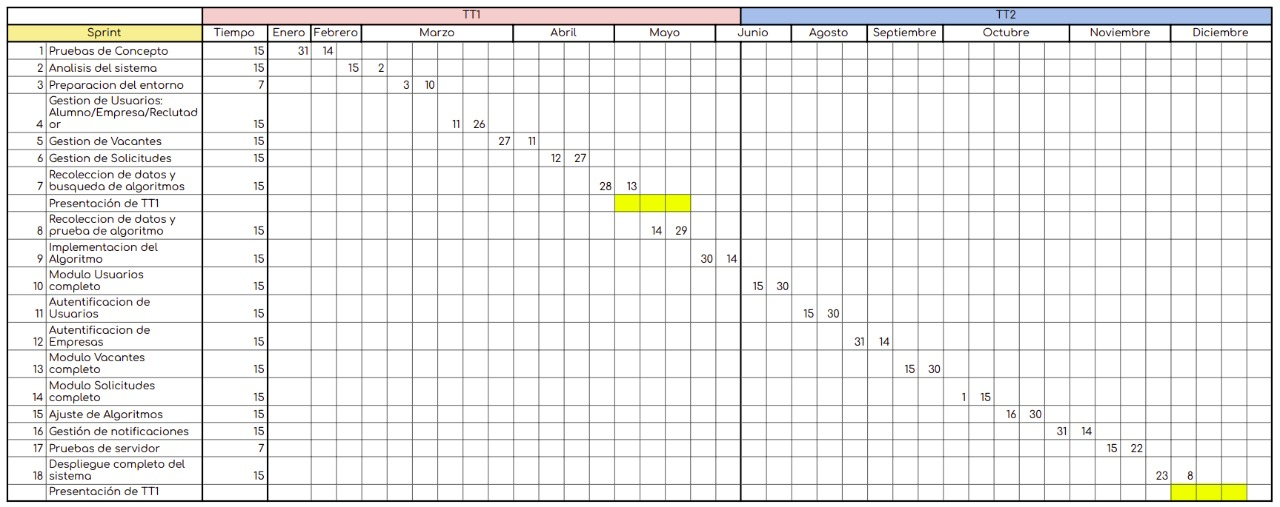
\includegraphics[width=1\textwidth]{propuesta/imagenes/gantt.jpeg}
    \end{center}
    \caption{Diagrama de Gantt del sistema}
    \label{fig:cronograma}
\end{figure}

En la entrega de TT1 los sprints que se van a ejecutar son:

\begin{itemize}
    \item \textbf{Sprint 1}: Pruebas de Concepto.
    \item \textbf{Sprint 2}: Analisis del sistema.
    \item \textbf{Sprint 3}: Preparacion del entorno.
    \item \textbf{Sprint 4}: Gestion de Usuarios: Alumno/Empresa/Reclutador.
    \item \textbf{Sprint 5}: Gestion de Vacantes.
    \item \textbf{Sprint 6}: Gestion de Solicitudes.
    \item \textbf{Sprint 7}: Recoleccion de datos y busqueda de algoritmos.
\end{itemize}


En la entrega de TT2 los sprints que se van a ejecutar son:

\begin{itemize}
    \item \textbf{Sprint 8}:  Recoleccion de datos y prueba de algoritmo.
    \item \textbf{Sprint 9}:  Implementacion del Algoritmo.
    \item \textbf{Sprint 10}: Modulo Usuarios completo.
    \item \textbf{Sprint 11}: Autentificacion de Usuarios. 
    \item \textbf{Sprint 12}: Autentificacion de Empresas.
    \item \textbf{Sprint 13}: Modulo Vacantes completo.
    \item \textbf{Sprint 14}: Modulo Solicitudes completo.
    \item \textbf{Sprint 15}: Ajuste de Algoritmos.
    \item \textbf{Sprint 16}: Gestión de notificaciones.
    \item \textbf{Sprint 17}: Pruebas de servidor.
    \item \textbf{Sprint 18}: Despliegue completo del sistema.
\end{itemize}
